\chapter{Testing} % Chapter 2
%


%\nocite{*}

\section{Introduction} % a.
This chapter looks at the results from training, testing and optimizing of the SVM Model selection process, in Section~\ref{sec:svm}. Table \ref{table: terms} gives an overview of the formulas and terms used in Figure ~\ref{fig:conf} and Table \ref{table:class} to describe the results.
\begin{table}[H]
\centering
\resizebox{\textwidth}{!}{
\begin{tabular}{ |c||c|c|}
	\hline
	\multicolumn{3}{|c|}{\textbf{SVM Model Evaluation}}\\
	\hline
      	\textbf{Term} &  \textbf{Formula} & \textbf{Description}\\
	\hline
      	\textbf{Type I Error} &      FP  &    False Positive   \\
	\hline
   	\textbf{Type II Error} &     FN  &    False Negative \\
	\hline
       	\textbf{Accuracy} &  $\frac{TP+TN}{TP+TN+FP+FN}$ & Evaluates the degree of correctness for the predictions   \\
	\hline
      	\textbf{Precision} &  $\frac{TP}{TP+FP}$ 	 &   The Positive predictive value \\
	\hline
    	\textbf{Recall} &     $\frac{TP}{TP+FP}$	 &   True positive rate  \\
	\hline
        \textbf{F1-Score} &  $2\times\frac{precision \times recall}{precision+recall}$  &   Evaluates the accuracy of predictions \\
	\hline
\end{tabular}}
\caption{Terminology and formulas used for evaluating the SVM Model \cite{dict}}
\label{table: terms}
\end{table}

%The testing of the entire system is followed in Section~\ref{sec:ahed}.

\subsection{Analysis of SVM Testing Results}\label{sec:svm}
The test set for testing the SVM model consisted of 136 entries, which is 40\% of the initial CK+ dataset. The overall accuracy of the SVM Model is 88.2\%, across all subjects and emotions. Table \ref{table:class} contains the `SVM Model Classification Report'. The report indicates the performance of each individual class, or emotion, and the overall estimated performance of the SVM model with regards to the precision, recall and f1-score. Classes that had more data available performed better overall as compared to those that had less. Since there was more testing data available for these classes. Working with an uneven dataset, see Figure~\ref{fig:pie}, makes it harder to judge the performance of each class in comparison to the other classes. 
\begin{figure}[H]
  \centering
  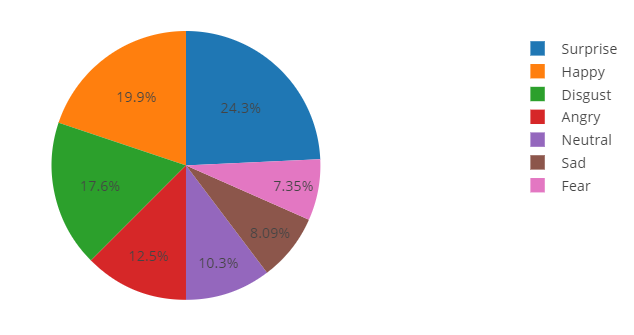
\includegraphics[scale=1.0]{pie}
  \caption{SVM test set breakdown}
  \label{fig:pie}
\end{figure} 
The emotions labelled \textit{Disgust, Happy} and \textit{Surprise} had over 24 subjects in the test set. This resulted in a higher f1-score for prediction accuracy of these emotions. Where the emotions labelled \textit{Sad, Neutral, Fear} and \textit{Angry} had significantly lower f1-score and fewer subjects in the test set. 
\begin{table}[H]
\centering
\resizebox{\textwidth}{!}{
\begin{tabular}{ |c||c|c|c|c|}
	\hline
	\multicolumn{5}{|c|}{\textbf{SVM Model Classification Report}}\\
	\hline
      	\textbf{Label} &      \textbf{precision} &   \textbf{recall} & \textbf{f1-score} &  \textbf{support}\\
	\hline
      	\textbf{Angry} &      0.74  &    0.82  &    0.78  &      17\\
   	\textbf{Disgust} &      1.00  &    0.92  &    0.96  &      24\\
       	\textbf{Fear} &      0.86  &    0.60  &    0.71  &      10\\
      	\textbf{Happy} &      0.93  &    1.00  &    0.96  &      27\\
    	\textbf{Neutral} &      0.67  &    0.71  &    0.69  &      14\\
        \textbf{Sad} &      0.75  &    0.82  &    0.78  &      11 \\
   	\textbf{Surprise} &      1.00  &    0.97  &    0.98  &      33 \\
	\hline
	\textbf{Avg \/ Total}  &     0.89 &     0.88  &   0.88    &   136\\
	\hline
\end{tabular}}
\caption{SVM Classification Report}
\label{table:class}
\end{table}


\subsection{Analysis of Confusion Matrix for Test Results}
The results from the confusion matrix, Figure ~\ref{fig:confu}, indicate that the model confuses the classes `Anger' and `Neutral' with each other. Out of the 5 misclassifications for the class `Neutral' 3 of them were for `Anger', and  2 of the 4 misclassifications for the class `Anger' were actually `Neutral'. The third class with a higher total for misclassifications was `Sad' with 3 misclassifications, 2 of them being `Fear'. Other classes had lower or no misclassifications for the given test set. This shows us that SVM the model is reasonably stable. 
\begin{figure}[H]
  \centering
  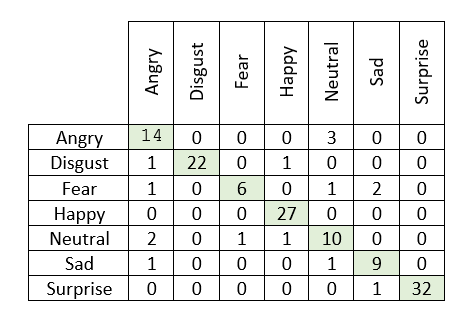
\includegraphics[scale=1.5]{conf1}
  \caption{Confusion Matrix of SVM Model Classification}
  \label{fig:confu}
\end{figure} 


\subsection{Analysis of SVM Testing Results for Subjects}
The results in the table,In Figure ~\ref{fig: res1} and ~\ref{fig: res2}, look at all the individual subjects within the test set and their classification performance using the SVM model. The original CK+ dataset is uneven in that not all subjects had all seven emotions present in the dataset. This made it challenging to split the dataset evenly based on subjects. The split was done by ensuring that each emotion had the same test-train ratio for the training dataset and the testing dataset. In the results table, the green represents a correct classification under the indicated "Emotion Label" and the red blocks indicate a misclassification for that emotion and the misclassification is included in white text. Each subject had at least one emotion classified during testing, with a maximum of five emotions for subject 'S055'. 

\begin{figure}[H]
  \centering
  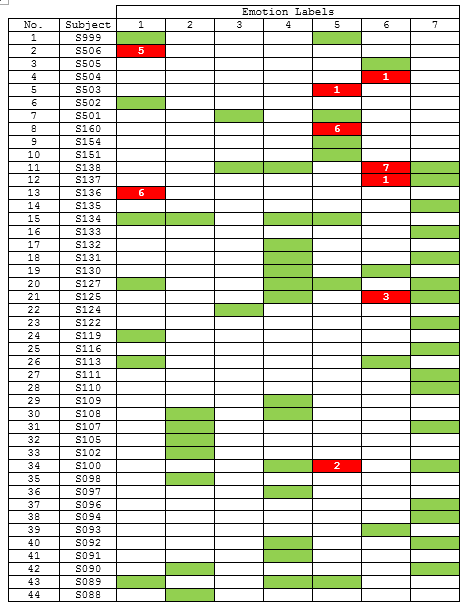
\includegraphics[scale=1.5]{res1}
  \caption{SVM Testing and Training Results for Subjects}
  \label{fig: res1}
\end{figure} 
\begin{figure}[H]
  \centering
  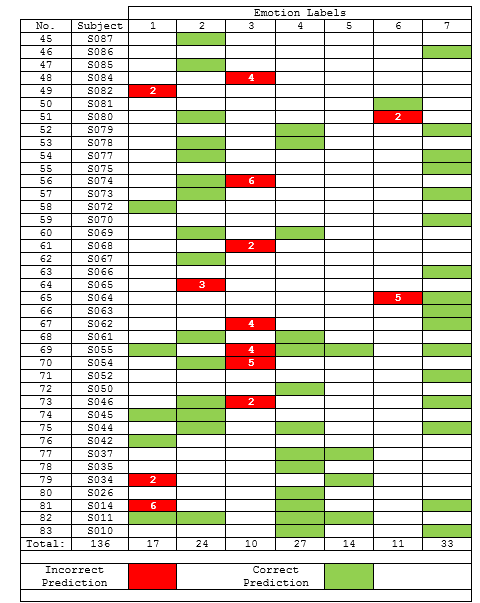
\includegraphics[scale=1.5]{res2}
  \caption{SVM Testing and Training Results for Subjects}
  \label{fig: res2}
\end{figure} 


\section{Conclusion}
The overall accuracy result for the SVM model was strong and generalized well with unseen data. Taking in to consideration that dataset used was not even, a further unbiased analysis on the results for individual subjects in the dataset was not possible. The dataset was split with the intention of having an equal ratio of subjects for each class in the testing set and the trainging set. As a result of this split analyzing the test results under each class proved to be more logical.

%\clearpage

%\subsection{Testing of AHED System}\label{sec:ahed}






